\prompt{Fit the spring data to a two-parameter Weibull distribution with shape parameter $k$ and scale parameter $\lambda$ using three optimization techniques:
Step-wise Gradient Descent,
Stochastic Gradient Descent,
and the Newton-Raphson Method.}



\begin{figure}[ht]
    \centering
    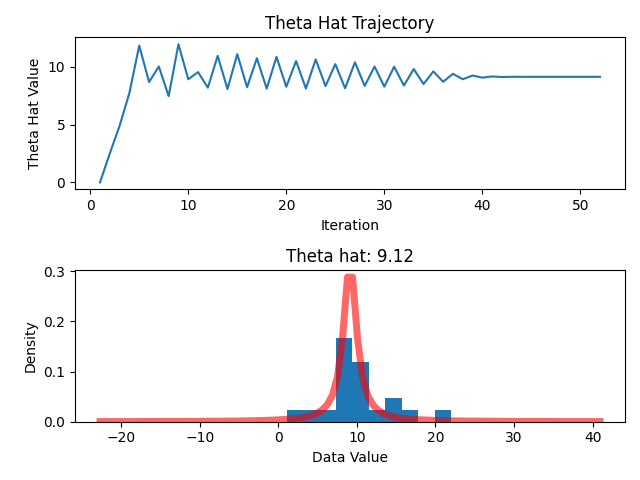
\includegraphics[width=0.5\textwidth]{figs/cauchy_swgd.png}
    \caption{Step-wise Gradient Descent}
    \label{fig:cauchy_swgd}
\end{figure}

Figure \ref{fig:cauchy_swgd} shows the optimization trajectory and fit using Step-wise Gradient Descent. 
I used an initial learning rate of .5 and used a decay schedule of $.999^{step}$ where $step$ was the number of optimization steps taken so far.
As you can see from the figure, the algorithm quickly got very close to the optimal setting, but oscillated around that for about 30 iterations/epochs.


\begin{figure}[ht]
    \centering
    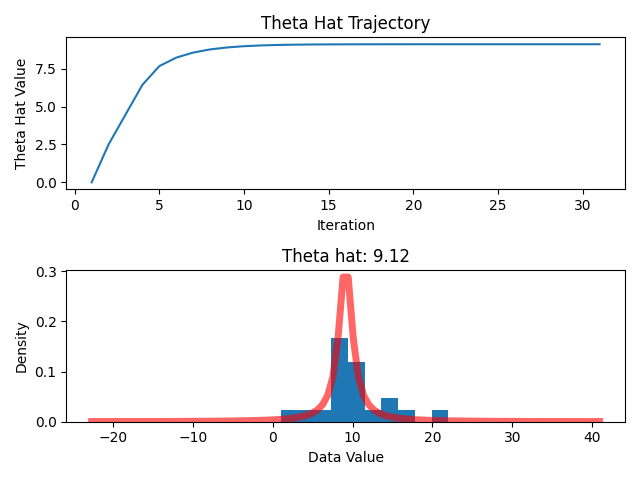
\includegraphics[width=0.5\textwidth]{figs/cauchy_nr.png}
    \caption{Newton-Raphson}
    \label{fig:cauchy_nr}
\end{figure}

Figure \ref{fig:cauchy_nr} shows the optimization trajectory and fit using the Newton-Raphson Method. 
This algorithm converged the quickest and did not oscilate which made each update highly targeted.

\begin{figure}[ht]
    \centering
    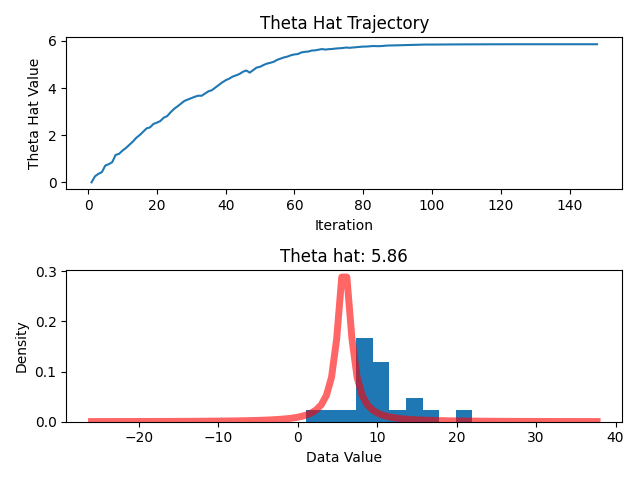
\includegraphics[width=0.5\textwidth]{figs/cauchy_sgd.png}
    \caption{Stochastic Gradient Descent}
    \label{fig:cauchy_sgd}
\end{figure}



Figure \ref{fig:cauchy_sgd} shows the optimization trajectory and fit using the Stochastic Gradient Descent. 
This algorithm took longer to converge than the others in terms of update steps (~80), but considering that updates were made for each data point instead of the entire dataset (20 data points), the covergence was quite fast in terms of epochs.
However, as you can see from the figure it did not obtain a very good fit.
This was likely due to the rate of decay. 
When I flattened the decay rate, the estimate became better, but the algorithm often took well over 1000 iterations to converge.

Also, with the current settings there wer no oscillations.
However, by the time the algorithm closed in on the correct solution the learning rate was much smaller (it was around .04 at iteration 70).
If the learning rate had been larger at that point I would expect to see the same sort of oscillations present in Step-wise Gradient Descent.


